% Created 2020-07-31 vie 11:49
% Intended LaTeX compiler: pdflatex
\documentclass[presentation,aspectratio=169]{beamer}
\usepackage[utf8]{inputenc}
\usepackage[T1]{fontenc}
\usepackage{graphicx}
\usepackage{grffile}
\usepackage{longtable}
\usepackage{wrapfig}
\usepackage{rotating}
\usepackage[normalem]{ulem}
\usepackage{amsmath}
\usepackage{textcomp}
\usepackage{amssymb}
\usepackage{capt-of}
\usepackage{hyperref}
\usepackage{khpreamble}
\usepackage{amssymb}
\usepgfplotslibrary{groupplots}
\newcommand*{\shift}{\operatorname{q}}
\usetheme{default}
\author{Kjartan Halvorsen}
\date{\today}
\title{Control computarizado - cierre}
\hypersetup{
 pdfauthor={Kjartan Halvorsen},
 pdftitle={Control computarizado - cierre},
 pdfkeywords={},
 pdfsubject={},
 pdfcreator={Emacs 26.3 (Org mode 9.3.6)}, 
 pdflang={English}}
\begin{document}

\maketitle


\section{Retroalimentación examen final}
\label{sec:org0163bc2}


\begin{frame}[label={sec:org8d832b1}]{Retroalimentación examen final}
\begin{itemize}
\item Comportamiento del sistema depende de la ubicación de polos en el plano z
\item Polos del observador
\begin{itemize}
\item El \alert{Observador} y sus polos tiene el mismo significado en control polinomial (RST) como en espacio de estado
\item La \alert{función de sensibilidad} tiene los polos del observador \alert{y} los polos de la respuesta al referencia \(\Rightarrow\) Se puede modificar con los polos del observador, pero dentro límites.
\end{itemize}
\end{itemize}
\end{frame}

\section{Retroalimentacion Tarea 5}
\label{sec:orge2a87ec}

\begin{frame}[label={sec:orgf52f999}]{Retroalimentación Tarea 5}
\begin{itemize}
\item Control por retroalimentación de estados (medidos o reconstruidos) \alert{no da acción integral}.
\item Se puede \alert{complementar} el control por retroalimentación de estados con acción integral.
\end{itemize}
\end{frame}

\section{Cierre}
\label{sec:org5488f81}


\begin{frame}[label={sec:orgaab05c4}]{Control en tiempo continuo}
\begin{center}
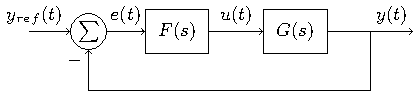
\includegraphics[width=0.6\linewidth]{../../figures/block1}
\end{center}
\end{frame}


\begin{frame}[label={sec:org9038dbb}]{Control en la vida real}
\begin{center}
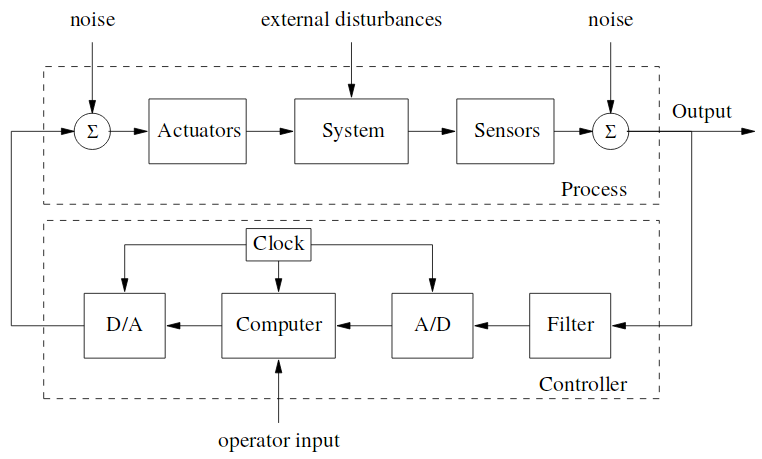
\includegraphics[width=0.7\linewidth]{../../figures/comp-contr-sys.png}
\end{center}
\footnotesize From Åström and Murray \emph{Feedback systems: An introduction for scientists and engineers}
\end{frame}

\begin{frame}[label={sec:org8140e86}]{Dos maneras de obtener un controlador discreto}
\begin{enumerate}
\item Discretizar un controlador diseñado usando métodos de tiempo continuo
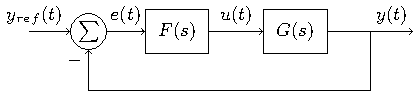
\includegraphics[width=0.7\linewidth]{../../figures/block1} \(F_d(z) \approx F(s)\)
\item Diseñar usando modelo discreto de la planta
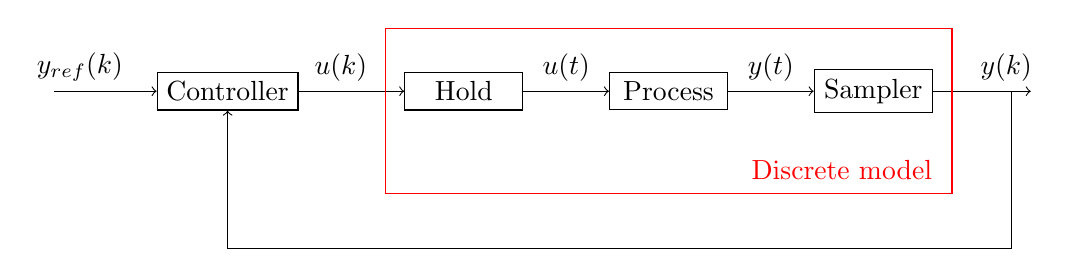
\begin{tikzpicture}[node distance=22mm, block/.style={rectangle, draw, minimum width=15mm}, sumnode/.style={circle, draw, inner sep=2pt}]

  \node[coordinate,] (refinput) {};
  \node[block, right of=refinput] (controller)  {Controller};
  \node[block, right of=controller, node distance=30mm] (zoh)  {Hold};
  \node[block, right of=zoh, node distance=26mm] (plant)  {Process};
  \node[block, right of=plant, node distance=26mm] (sampler)  {Sampler};
  \node[coordinate, right of=sampler, node distance=20mm] (output) {};

  \draw[->] (refinput) -- node[above, near start] {$y_{ref}(k)$} (controller);
  \draw[->] (controller) -- node[above, pos=0.4] {$u(k)$} (zoh);
  \draw[->] (zoh) -- node[above] {$u(t)$} (plant);
  \draw[->] (plant) -- node[above] {$y(t)$} (sampler);
  \draw[->] (sampler) -- node[pos=0.8, coordinate] (measure) {} node[above, near end] {$y(k)$} (output);
  \draw[->] (measure) -- ++(0,-20mm) -| (controller);
  \draw[red] (42mm, -13mm) rectangle (114mm, 8mm);
  \node[red] at (100mm, -10mm) {Discrete model};
\end{tikzpicture}
\end{enumerate}
\end{frame}

\begin{frame}[label={sec:orgbf9701c}]{Tiempo discreto vs tiempo continuo}
\begin{center}
\begin{tabular}{ll}
Continuous time & Discrete time\\
\hline
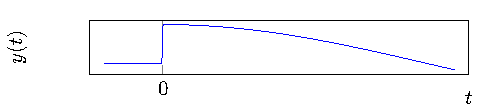
\includegraphics[width=0.4\linewidth]{../../figures/cont-fcn} & 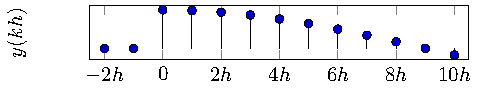
\includegraphics[width=0.4\linewidth]{../../figures/discrete-fcn}\\
\(y(t)\) & \(y(kh)\) or \(y(k)\)\\
\(\operatorname{p} y \triangleq \frac{d}{dt} y\) & \(\operatorname{q}y \triangleq y(kh+h)\)\\
\((\operatorname{p}+a) y = bu \;\Leftrightarrow\; \frac{d}{dt}y + ay = bu\) & \((\operatorname{q} + \alpha) y = \beta u \; \Leftrightarrow \; y(k+1) + \alpha y(k) = \beta u(k)\)\\
\(Y(s) \triangleq \laplace{y(t)}\) & \(Y(z) \triangleq \ztrf{y(kh)}\)\\
\(Y(s) = G(s)U(s) = \frac{b}{s+a}U(s)\) & \(Y(z) = H(z)U(z) = \frac{\beta}{z+\alpha}U(z)\)\\
Pole of the system: \(s+a=0 \; \Rightarrow \; s = -a\) & Pole of the system: \(z+\alpha = 0 \; \Rightarrow \; z = -\alpha\)\\
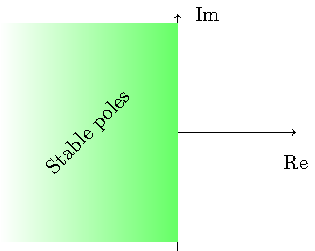
\includegraphics[width=0.22\linewidth]{../../figures/cont-stable} & 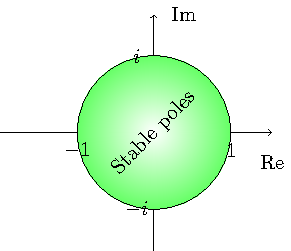
\includegraphics[width=0.22\linewidth]{../../figures/discrete-stable}\\
\hline
\end{tabular}
\end{center}
\end{frame}

\begin{frame}[label={sec:org171452c}]{Objetivos del curso}
Al final del curso serás capaz de:

\begin{enumerate}
\item \alert{Analizar} sistemas de control computarizado de procesos y productos.
\item \alert{Diseñar} sistemas de control computarizado de procesos y productos.
\item \alert{Implementar} sistemas de control computarizado de procesos y productos.
\item \alert{Evaluar} sistemas de control computarizado de procesos y productos con un enfoque de aplicación práctica.
\end{enumerate}
\end{frame}

\begin{frame}[label={sec:orgc76446b}]{}
\Huge Tusen takk
\end{frame}
\end{document}